\subsubsection{\label{API} API Package}
\paragraph{Package: api} This package is the interface between the client's application and the server application. 
All requests are sent to this API(package) in JSON format.

\class{FrontendAPI}

\begin{figure}[h]
        \centerline{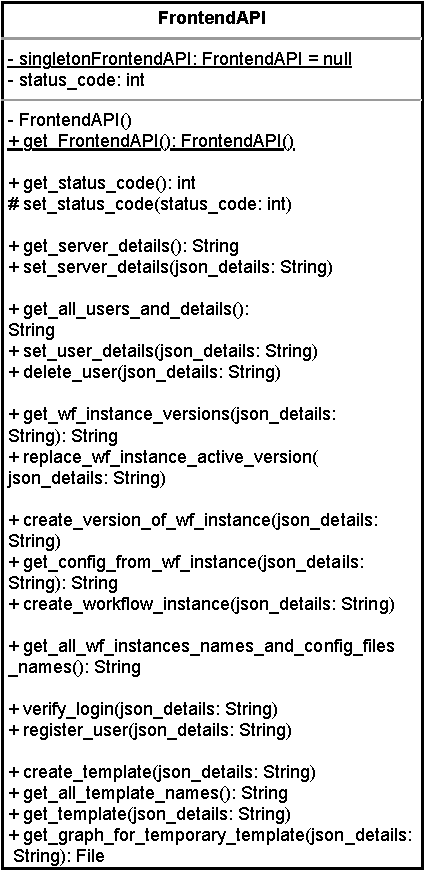
\includegraphics[scale=1]{res/Klassen/FrontendAPI.pdf}}
        \caption{FrontendAPI class from class diagram}
\end{figure}

This class is the main interface of the whole application. The client application
can get the api status code to obtain information regarding the execution of api calls (e.g. status code
changes when an exception has been thrown)

\begin{methodenv}{Methods}

\method{static get\texttt{\_}FrontendAPI(): FrontendAPI} returns the FrontendAPI in singleton design fashion, meaning 
there is only one instance of FrontendAPI in circulation at all times.

\method{get\texttt{\_}status\texttt{\_}code(): int} return status code  

\method{set\texttt{\_}status\texttt{\_}code(status\texttt{\_}code: int)}
sets the status code, only performed by the \textbf{ExceptionHandler}
\smallPara{Parameters}
\begin{itemize}
        \item \textbf{status\texttt{\_}code}
        the status code showing the state of the latest API call
\end{itemize}

\method{get\texttt{\_}server\texttt{\_}details(): String}
gets all server details (container limit, cpu resources, gpu resources, servername, ip address, executing server (yes/no)) 
and returns them in a json format 

\method{set\texttt{\_}server\texttt{\_}details(json\texttt{\_}details: String)}
sets all server details (container limit, cpu resources, gpu resources, servername, ip address, executing server (yes/no)) in
 a json format. Only one bulk update as a whole
due to long delay with server communication from client's perspective
\smallPara{Parameters}
\begin{itemize}
        \item \textbf{server\texttt{\_}details}
        all server details in json format
\end{itemize}

\method{get\texttt{\_}all\texttt{\_}users\texttt{\_}and\texttt{\_}details(): String}
gets all users and their details (user names, privileges, statuses) in a json format. Only one bulk update as a whole
due to long delay with server communication from client's perspective


\method{set\texttt{\_}all\texttt{\_}users\texttt{\_}and\texttt{\_}details(json\texttt{\_}details: String)}
sets all user details (user name, privilege, statuse) for a specific user in a json format. Only one bulk update as a whole
due to long delay with server communication from client's perspective. If user does not already exist, one will be created.

\method{delete\texttt{\_}user(json\texttt{\_}details: String)}
deletes a user by username
\smallPara{Parameters}
\begin{itemize}
        \item \textbf{json\texttt{\_}details}
        json object which only contains the username key and value
\end{itemize}


\method{get\texttt{\_}wf\texttt{\_}instance\texttt{\_}version\texttt{\_}number
(json\texttt{\_}details: String): String}
returns workflow instance's version number 
\smallPara{Parameters}
\begin{itemize}
        \item \textbf{json\texttt{\_}details}
        json object which only contains the workflow instance name and version number 
\end{itemize}

\method{replace\texttt{\_}wf\texttt{\_}instance\texttt{\_}version\texttt{\_}number
(json\texttt{\_}details: String)}
replaces the specified workflow instance's version number 
\smallPara{Parameters}
\begin{itemize}
        \item \textbf{json\texttt{\_}details}
        json object which only contains the workflow instance name and version number
\end{itemize}


\method{create\texttt{}version\texttt{\_}of\texttt{\_}wf\texttt{\_}instance(json\texttt{\_}details)}
changes multiple config files based on input/ key value pair changes in client's applications during workflow instance 
configuration
\smallPara{Parameters}
\begin{itemize}
        \item \textbf{json\texttt{\_}details}
        json object which contains the changed config files name, 
        all key value pairs per config file, 
        contains workflow instance name
\end{itemize}

\method{get\texttt{\_}config\texttt{\_}from\texttt{\_}wf\texttt{\_}instance(json\texttt{\_}details): String}
gets all config file names related to specific workflow instance (version)
\smallPara{Parameters}
\begin{itemize}
        \item \textbf{json\texttt{\_}details}
        json object which contains the wanted workflow instance name and its respective version and config file name
\end{itemize}


\method{get\texttt{\_}all\texttt{\_}wf\texttt{\_}instances\texttt{\_}names\texttt{\_}and\texttt{\_}config\texttt{\_}files
\texttt{\_}names(json\texttt{\_}details: String)}
gets all  config file and all workflow instances \textbf{names} 

\method{verify\texttt{\_}lgin(json\texttt{\_}details:String)}
verifies username with associated password
\smallPara{Parameters}
\begin{itemize}
        \item \textbf{json\texttt{\_}details}
        contains username and password
\end{itemize}

\method{register(json\texttt{\_}details:String)}
registers a new user
\smallPara{Parameters}
\begin{itemize}
        \item \textbf{json\texttt{\_}details}
        contains username, password and repeated password
\end{itemize}

\method{get\texttt{\_}graph\texttt{\_}for\texttt{\_}temporary\texttt{\_}template(json\texttt{\_}details:String): File}
gets a preview picture of the DAG (used when in editor preview mode)
\smallPara{Parameters}
\begin{itemize}
        \item \textbf{json\texttt{\_}details}
        contains encoded template
\end{itemize}

\method{create\texttt{\_}template(json\texttt{\_}details:String)}
creates a new template
\smallPara{Parameters}
\begin{itemize}
        \item \textbf{json\texttt{\_}details}
        contains encoded template
\end{itemize}

\end{methodenv}

%neue Klasse
\class{JSONToPython}

\begin{figure}[h]
        \centerline{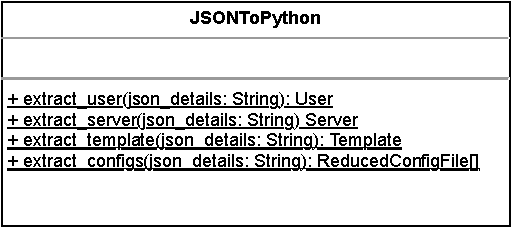
\includegraphics[scale=1]{res/Klassen/JSONToPython.pdf}}
        \caption{JSONToPython class from class diagram}
\end{figure}

This class converts all json data into the wanted object by extracting certain keys and values and instantiating
a new (temporary) object which executes the wanted methods (e.g. extract server and then execute set new container limit).
Instantiated objects will be deleted by the garbage collection after they are finished writing back / getting data
from the database.

\begin{methodenv}{Methods}

\method{static extract\texttt{\_}user(json\texttt{\_}details:String): User}
extracts json details and builds a new User based off of these json details
\smallPara{Parameters}
\begin{itemize}
        \item \textbf{json\texttt{\_}details}
        contains username, privilege and status
\end{itemize}

\method{static extract\texttt{\_}server(json\texttt{\_}details:String): Server}
extracts json details and builds a new Server based off of these json details
\smallPara{Parameters}
\begin{itemize}
        \item \textbf{json\texttt{\_}details}
        contains servername, container limit, cpu and gpu resources, executing server (yes/no) and ip address
\end{itemize}

\method{static extract\texttt{\_}template(json\texttt{\_}details:String): Template}
extracts json details and builds a new Template based off of these json details
\smallPara{Parameters}
\begin{itemize}
        \item \textbf{json\texttt{\_}details}
        contains dag definition file name and template name
\end{itemize}

\method{static extract\texttt{\_}configs(json\texttt{\_}details:String): ReducedConfigFile[]}
extracts json details and builds a new ReducedConfigFile array based off of these json details
\smallPara{Parameters}
\begin{itemize}
        \item \textbf{json\texttt{\_}details}
        contains config files names which in themselves contain config file name, workflow instance name,
        and key value pairs
\end{itemize}

\end{methodenv}

%neue Klasse
\class{PythonToJSON}

\begin{figure}[h]
        \centerline{\includegraphics[scale=1]{res/Klassen/PythonToJson.pdf}}
        \caption{PythonToJSON class from class diagram}
\end{figure}

This class converts all python objects into json data by extracting certain keys and values and dumping
them into a json object.

\begin{methodenv}{Methods}

\method{static encode\texttt{\_}user(user: User): String}
extracts all user attributes and dumps them into json object
\smallPara{Parameters}
\begin{itemize}
        \item \textbf{user}
        user whose attributes are to be encoded
\end{itemize}

\method{static encode\texttt{\_}server(server: Server): String}
extracts all server attributes and dumps them into json object
\smallPara{Parameters}
\begin{itemize}
        \item \textbf{user}
        server whose attributes are to be encoded
\end{itemize}

\method{static encode\texttt{\_}template(template: Template): String}
extracts template attributes and dumps them into json object
\smallPara{Parameters}
\begin{itemize}
        \item \textbf{user}
        template whose attributes are to be encoded
\end{itemize}

\method{static encode\texttt{\_}wf\texttt{\_}instance(wf\texttt{\_}instance: WorkflowInstance): String}
extracts workflow instance attributes and dumps them into json object
\smallPara{Parameters}
\begin{itemize}
        \item \textbf{user}
        workflow instance whose attributes are to be encoded
\end{itemize}

\method{static encode\texttt{\_}config(config: ReducedConfigFile): String}
turns key value pairs into json object
\smallPara{Parameters}
\begin{itemize}
        \item \textbf{user}
        config file whose attributes are to be encoded
\end{itemize}

\end{methodenv}

%neue Klasse
\class{Exception Handler}

\begin{figure}[h]
        \centerline{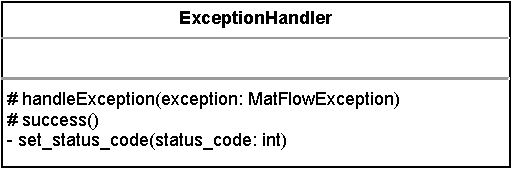
\includegraphics[scale=1]{res/Klassen/ExceptionHandler.pdf}}
        \caption{ExceptionHandler class from class diagram}
\end{figure}

This class handles all MatFlowExceptions and those who inherit from MatFlowException. It is  
responsible for changing the API's status code.

\begin{methodenv}{Methods}

\method{handle\texttt{\_}exception(exception: MatFlowException)}
sets the API's status code to the specific exception's status code by calling the private method
set\texttt{\_}status\texttt{\_}code.
\smallPara{Parameters}
\begin{itemize}
        \item \textbf{exception}
        specific MatFlowException that was thrown during request
\end{itemize}

\method{success()}
sets status code to success code

\end{methodenv}

